\documentclass[12pt, letterpaper]{article}
\usepackage{listings}
\usepackage{graphicx}
\usepackage{color}
\usepackage{caption}
\usepackage{subcaption}
\usepackage{hyperref}
\usepackage{fancyhdr}
\usepackage{mathrsfs}
\usepackage[margin=3cm]{geometry}
\usepackage[dvips]{epsfig}
\usepackage{placeins}
\setlength{\parindent}{0.0in}
\setlength{\parskip}{0.05in}

\definecolor{dkgreen}{rgb}{0,0.6,0}
\definecolor{gray}{rgb}{0.5,0.5,0.5}
\definecolor{mauve}{rgb}{0.58,0,0.82}
\definecolor{deepblue}{rgb}{0,0,0.7}
\definecolor{deepred}{rgb}{0.6,0,0}
\definecolor{deepgreen}{rgb}{0,0.5,0}
\definecolor{red}{rgb}{0.9,0,0}

\newcommand\course{CS532}
\newcommand\semester{Spring 2017}
\newcommand\hwnum{4}
\newcommand\yourname{Justin Schaffner}
\newcommand\login{JASchaff}
\newenvironment{answer}[1]{\subsection*{Problem #1}}

\pagestyle{fancyplain}
\headheight 40pt
\lhead{\yourname\ (\login)\\\course\ --- \semester}
\chead{\textbf{\Large Assignment \hwnum}}
\rhead{\today}
\headsep 40pt
\lstnewenvironment{MyBash}{\lstset{language=bash, aboveskip=3mm, belowskip=3mm, showstringspaces=false, columns=flexible, basicstyle={\small\ttfamily}, numbers=none, numberstyle=\tiny\color{grey}, keywordstyle=\color{black}, commentstyle=\color{dkgreen}, stringstyle=\color{black}, breaklines=true, breakatwhitespace=true, tabsize=3}}{}
\lstnewenvironment{MyPython}{\lstset{language=Python, aboveskip=3mm, belowskip=3mm, basicstyle=\small, otherkeywords={self}, keywordstyle=\color{deepblue}, emph={MyClass,__init__}, emphstyle=\color{deepred}, stringstyle=\color{deepgreen}, commentstyle=\color{red}, frame=tb, showstringspaces=false, breaklines=true }}{}
\lstnewenvironment{MyR}{\lstset{language=R, aboveskip=3mm, belowskip=3mm, basicstyle=\small, breaklines=true}}{}

\begin{document}

\begin{answer}{1: Friendship Paradox on Facebook}
Question 1: Determine if the friendship paradox holds for M. Nelson's Facebook
account. Compute the mean, standard deviation, and median of the
number of friends that M. Nelson's friends have. Create a graph of the
number of friends (y-axis) and the friends themselves, sorted by
number of friends (x-axis).Do include M. Nelson in the graph
and label him accordingly.
For this exercise I used R to import the graphml document of M. Nelsons facebook network. Due to the number of friends, I flipped the x and y axis so that the names would be to the left, and readable. M. Nelson's friend count is highlighted in blue. The mean, median and standard deviation are also calculated using R, and the n rounded to 3 significant digits. \\
Here is the R code used to generate the graph:\\
\begin{MyR}
require(graphics)
library(igraph)
library(ggplot2)

pdf('Desktop/facebook_friend_paradox.pdf')
facebook_graph<-read.graph('Desktop/mln.graphml', format='graphml')
name<-V(facebook_graph)$name
friend_count<-V(facebook_graph)$friend_count

FB_frame<-data.frame(name=name, friend_count=friend_count, color='blue') 	#build data frame from attribute vectors
FB_frame<-na.omit(FB_frame)	#remove missing data
summary(FB_frame)	#show a summary of the data

max_friends<-max(FB_frame$friend_count) #calculate the largest number of friends a friend has
class(max_friends)

num_friends<-length(FB_frame$friend_count) #calculate the total number of friends
class(num_friends)

dev_f<-as.integer(sd(FB_frame$friend_count)+0.5) #calculate the standard deviation
class(dev_f)

mean_f<-as.integer(mean(FB_frame$friend_count)+0.5) #calculate the mean
class(mean_f)

median_f<-as.integer(median(FB_frame$friend_count)+0.5) #calculate the median
class(median_f)

temp<-data.frame(name='Michael Nelson', friend_count=num_friends, color='red') #add M. Nelson to the data frame but colored red
FB_frame<-rbind(FB_frame, temp)
summary(FB_frame)

num_friends<- num_friends + 1
FB_frame$name<-factor(FB_frame$name, levels=FB_frame[order(FB_frame$friend_count), 'name']) #reorder the data table for smallest to largest 

ggplot(FB_frame, aes(x=name, y=friend_count, colour=color)) + geom_bar(stat='identity') + coord_flip()+ theme(axis.text=element_text(size=3.5), legend.position='none')+xlab('Friend Count')+ylab('Friends')+ggtitle('Freindship Paradox')+annotate('text', x= c(90, 85, 80, 75, 70, 65, 60, 55), y=2000, label=c('Mean: ', mean_f,'Median: ', median_f, 'Stan Dev: ',  dev_f, 'Total Friends: ', num_friends-1) )
dev.off()
\end{MyR}
I'm not sure why, but when the graph was built, the colors switched, so that M. Nelson is highlighted blue, while everyone else is red. I'll figure that out for next time, but at least the right data point still stands out. \\
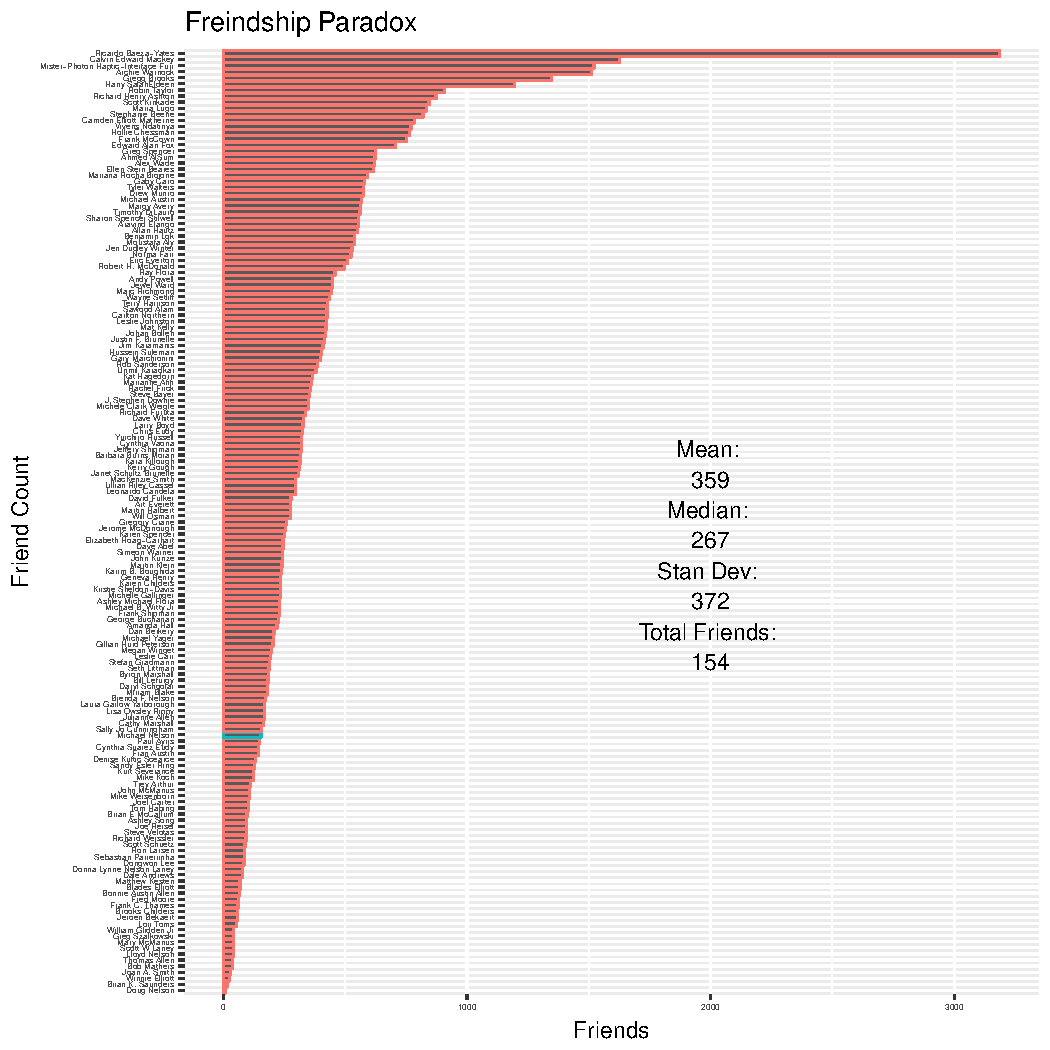
\includegraphics[width=\linewidth]{facebook_friend_paradox}
The data suggests that yes, most of M. Nelson's friends have more friends than he does, proving the Friendship paradox. This is represented by the median vs. the total number of friends.

\end{answer}
\begin{answer}{2: Friendship Paradox on Twitter}
Determine if the friendship paradox holds for the phonedude\textunderscore mln Twitter account.
Since Twitter is a directed graph, use "followers" as the value you measure.
For this problem, I built a quick Python program to query Twitter called ``Twitter\textunderscore Followers.py". I used Python 3.5, and the program takes two arguments. The first is the output file for the data, and the second is the screen name of the profile you wish to query. The program creates a tabulated file with two columns: the screen name of the follower, and the number of followers they have. \\
Here is the code for ``Twitter\textunderscore Followers.py":
\begin{MyPython}
#Import the necessary methods from tweepy library
import tweepy
import json
import re as regex
import requests
from sys import argv

#Variables that contains the user credentials to access Twitter API 
access_token = "826264224838057986-p2cjKY6P4qKUUbTRtDZDicIHFxXkCdu"
access_token_secret = "yTAtL6R0rb35p49qcharmzWMz5X4vQsT0Jrm2UQR7Nipf"
consumer_key = "1qH36csH37Oa1LKjgDijsxGVX"
consumer_secret = "QlVfb24OuyOGsMmF8ojWZs1N2p1eeT8ib2CK4ovntk1tpSLIaW"

if __name__ == '__main__':
    outfile=argv[1]
    screenname=argv[2]
    #creates authentication object using pasted tokens and keys
    auth = tweepy.OAuthHandler(consumer_key, consumer_secret)
    auth.set_access_token(access_token, access_token_secret)
    #I added the wait_on_rate_limit and notify flags. this keeps the program from
    #crashing when Twitter raises the rate_limit_exceeded flag. Wish I'd known about
    #that last time!
    api=tweepy.API(auth, wait_on_rate_limit=True, wait_on_rate_limit_notify=True)
    
    with open(outfile, 'w') as out:
        print('screen_name', 'followers', sep='\t', file=out)
        #iterable object c pulls followers from a particular user
        c=tweepy.Cursor(api.followers, screen_name=screenname).items()
        while True:
            try:
                user= c.next()
                #using the tweepy API you can pull screen_name and followers_count
                #from a particular user
                print(user.screen_name, user.followers_count, sep='\t', file=out)
                #I added this error catch before I found the flags above.
            except tweepy.TweepError:
                continue
            except StopIteration:
                break
\end{MyPython}
Here is the R code used to draw the graph:\\
\begin{MyR}
require(graphics)
pdf('Desktop/Twitter_Friend_Paradox.pdf')

twit_frame<-read.table('Desktop/twitter_follow.txt', sep='\t', header=TRUE) 	#import frame from file
twit_frame<-na.omit(twit_frame)	#remove NA
twit_frame$color<-'blue'	#add color column
twit_frame$size<-0.01	#add size column

max_followers<-max(twit_frame$followers)	#calculate max number of followers a follower has
class(max_followers) 	#checks max followers for type

num_followers<-length(twit_frame$followers) #calculate total number of followers
class(num_followers)

dev_f<-as.integer(sd(twit_frame$followers)+0.5)	#calculates standard deviation
class(dev_f)

mean_f<-as.integer(mean(twit_frame$followers)+0.5)	#calculates the mean
class(mean_f)

median_f<-as.integer(median(twit_frame$followers)+0.5)	#calculates the median
class(median_f)

summary(twit_frame)	#displays a summary of twit_frame so far
temp<-data.frame(screen_name='phonedude_mln', followers=num_followers, color='red', size=0.5)	#crates a row for phonedude_mln
twit_frame<-rbind(twit_frame, temp)	#adds phonedude_mln to twit_frame
summary(twit_frame)
num_followers<- num_followers + 1	#adds one more to the row count for use while plotting

twit_frame$screen_name<-factor(twit_frame$screen_name, levels=twit_frame[order(twit_frame$followers), 'screen_name'])	#reorders twit_frame smallest to largest

ggplot(twit_frame, aes(x=screen_name, y=followers, colour=color, size=size)) + geom_bar(stat='identity') + coord_flip()+ theme(axis.text=element_text(size=0.01), axis.text.x=element_text(size=10), legend.position='none')+xlab('Followers')+ylab('Follower Count')+ggtitle('Freindship Paradox on Twitter')+annotate('text', x= c(500, 480, 460, 440, 425, 410, 395, 380), y=50000, label=c('Mean: ', mean_f,'Median: ', median_f, 'Stan Dev: ',  dev_f, 'Total Followers: ', num_followers-1) )
dev.off()
\end{MyR}
For the plot, I basically used the same code as the previous graph, but I added a size varibale so I could blow up M. Nelson's bar. The regular plot almost disappeared otherwise. I also suppressed the screen names as much as possible since it was too crowded to be readable.\\
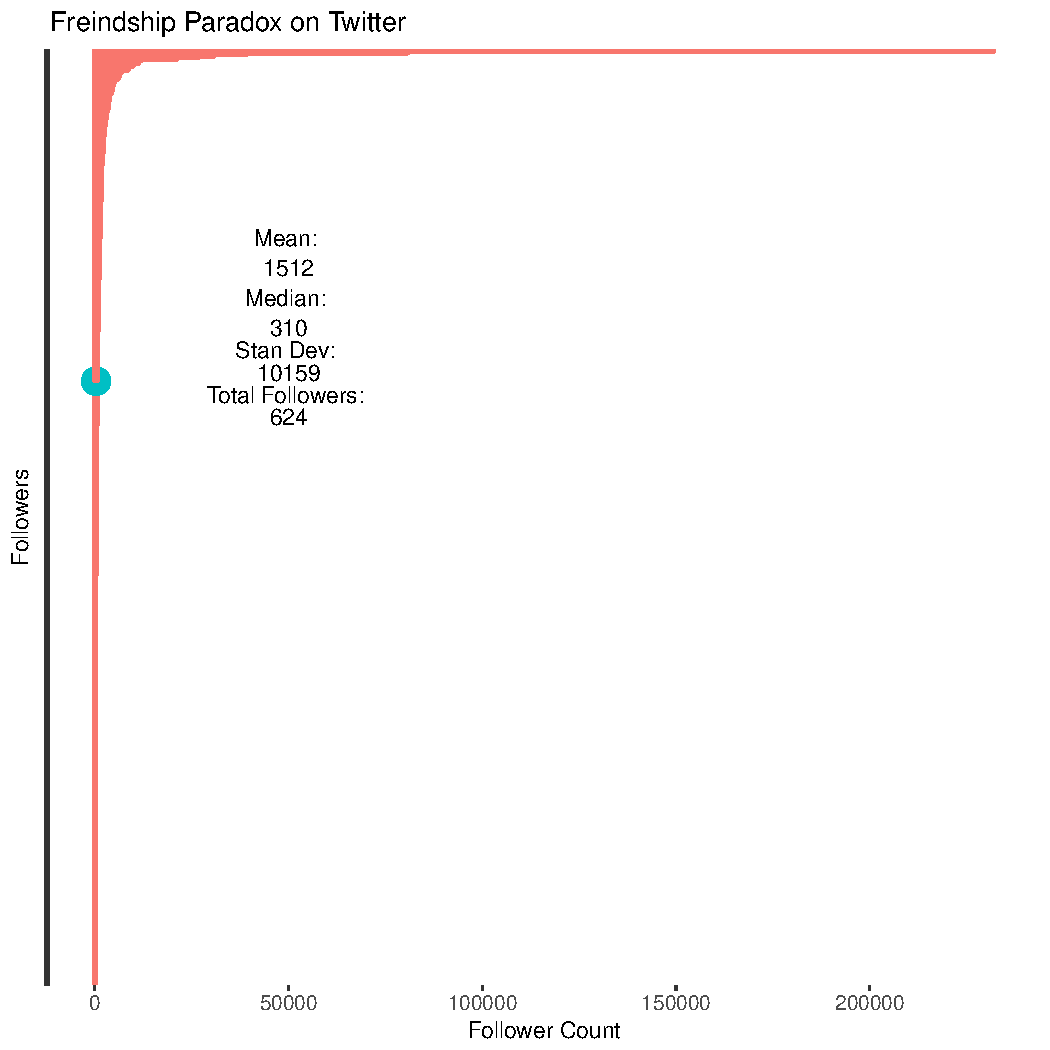
\includegraphics[width=\linewidth]{Twitter_Friend_Paradox}
The data on this graph suggests that most of M. Nelson's followers have LESS followers than he does, as represented by the median vs. the total number of followers

\end{answer}

\end{document}